\newchap{Representations of Written and Spoken Language}
\label{chap:ling-background}

From a linguistic point of view there are two high-level concepts that are important for this thesis. The first and most significant one is that of the \textbf{relation of written and spoken language}. Both spoken and written language are a way of representing a language in general. I would like to find out what traditional linguistics states about the relation of written and spoken language. Both written and spoken language are \textit{valid} representations of the same language. As we will see later in this chapter, mapping a spoken language to its written representation is far from easy and never perfect. Elaborated writing systems like we are used to today came only much later compared to language in general\myfootnote{\url{https://www.youtube.com/watch?v=-sUUWyo4RZQ&list=PL8dPuuaLjXtP5mp25nStsuDzk2blncJDW&index=18}} \citep{Hock&Joseph.2019}. 

Whenever we study language we look at samples of that language. It is simply impossible to study an \textit{entire} language as we would need all texts that were ever produced in that language. Consequently, we need to ask ourselves how much and what material of a language is enough, to study it properly. In order to do that we can make use of techniques and methods from corpus linguistics. In linguistics and also in computational linguistics we typically talk about a corpus when we talk about a huge dataset that is used to represent a language. It does not matter if the corpus contains written or spoken samples of a language although it is mostly written \citep{McEnery&Hardie.2011}. Corpus linguistics allows for both qualitative and quantitative analysis of text. Due to recent technological advancement it has become possible to store large digital collections of speech recordings and their aligned transcriptions. These possibilities gave rise to a wider acknowledgement of corpus phonetics. Corpus phonetics deals with an abundance of linguistic variation. In addition to language, style or vocabulary variation, there are differences in dialect and idiolect, physiological state of the speakers and their attitude \citep{Liberman.2019, Chodroff.19.07.2019}. In section \ref{nws}, I will present an interesting study on corpus phonetics \citep{baird_evans_greenhill_2021}. The authors of the study aim to answer how much phonetic data is needed to cover all sounds of a language.

The second key concept is that of \textbf{multilingual analysis}. The corpus underlying this thesis is multilingual. I will introduce this corpus later in section \ref{sec:corpus}. While a multilingual corpus in itself is not uncommon, the specific goal of the team maintaining the corpus is to compare the languages and study their similarities. Comparing languages and studying their similarities and differences is part of a well-established branch of traditional linguistics called comparative linguistics. For example, \citet{gutierrez-vasques-etal-2021-characters} performed a study on a multilingual corpus comparing different subword tokenizations. They compared 47 languages to find out how languages can be tokenized such that it leads to similar distributions among that languages. This analysis was performed on written language and is an example for what could be done on a phonetic corpus as well.

While there is a lot that could be said about any of these topics, I am not going into more detail about these. The point I would like to make is that the task of creating phonetic transcriptions of a multilingual corpus with the long-term objective of comparing written and spoken language is deeply rooted in linguistics and not at all trivial. In the following sections I will mostly write about phonetics and phonology in general and writing systems.

\section{Phonetics and phonology}
\label{phonetics}
Given that phonetics and phonology is a sub-area of traditional linguistics and often only touched on superficially in computational linguistics, I will summarise the most important assumptions and terms that are necessary to understand what phonetic transcriptions are.
A very important terminological distinction is between \textbf{phonetics} and \textbf{phonology}. While phonetics refers to the study of actual sounds, phonology refers to the study of sound \textit{systems}. In phonetics, it is not so much important what the different sounds mean, but how they are produced and perceived and what different sounds a human being can produce and perceive at all. When it comes to human communication using spoken language, many sounds that can be produced are not actually meaningful. A human being is perfectly capable of producing many different sounds but some just do not mean anything to other people. The study of sound systems, phonology, is used to describe the set of sounds that make up a language. The sounds within a sound system of a language can be used to construct meaningful utterances. For this thesis, phonology is more important.

Example \ref{ex:phon} shows how the word `request' can be pronounced in English. The pronunciation is written in the \ac{ipalpha} which I will explain in more depth in section \ref{sec:ipa}. For now it is important to note that the same word can be pronounced differently.

\begin{covsubexamples}[preamble={Different pronunciations of the English word `request' (except for the last example). The spaces indicate how the letters can be mapped to the phonetic symbols on the right side:}] \label{ex:phon}
\item \label{ex:phonetics} r e qu e s t $\rightarrow$ [\textipa{\*r I kw E s t}] %ɹ ɪ kw ɛ s t
\item \label{ex:phonetics2} r e qu e s t $\rightarrow$ [\textipa{R I kw E s t}] %ɻ̥ ɪ  w ɛ s t 
\item \label{ex:phonetics3} r e qu e s t $\rightarrow$ [\textipa{r I kw E s t}] %r ɪ k w ɛ s tt 
\item \label{ex:phonetics4} b e qu e s t $\rightarrow$ [\textipa{b I kw E s t}] %r ɪ k w ɛ s t
\end{covsubexamples}

Example \ref{ex:phonetics} shows how the word `request' is pronounced in British English. Even someone that does not know the \ac{ipalpha} can see that the letter `r' can be mapped to the pronunciation symbol [\textipa{\*r}]. Another English speaker might pronounce the letter `r' a bit different as in example \ref{ex:phonetics2}. We can see that the pronunciation symbol [\textipa{R}] for the `r' differs from the one in the first example. 
However, an English speaker would still understand the word `request' as the different pronunciation does not change the meaning of the word. In phonetic terms we would say that in the British English sound system there exists an abstract sound /\textipa{\*r}/ which is called the \textbf{phoneme} /\textipa{\*r}/. Note that we write a phoneme between slashes. 
Also, in our case there exist two \textbf{phones} [\textipa{\*r}] and [\textipa{R}] which are specific sounds that can be used to pronounce the phoneme /\textipa{\*r}/. No matter which phone I use, it does not change the meaning of the word. Note that we write a phone between square brackets. In British English, [\textipa{R}] is an \textbf{allophone} of the phoneme /\textipa{\*r}/. 
Allophones are specific phones that are concrete realizations of the same phoneme. Realization in this case just means that it is a sound in an actual utterance. Allophones of the same phoneme can be used interchangably without changing the meaning of the utterance. Very importantly, allophones are language specific. In other languages I cannot use the same phones to pronounce a phoneme. In example \ref{ex:phonetics3}, the `r' is mapped to the phone [\textipa{r}] which is part of the Spanish sound system. [\textipa{r}] is not an allophone of /\textipa{\*r}/ in British English as typically British English speakers do not say the `r' like in Spanish. The phone [\textipa{r}] does not exist in the British English sound system. Still, a British English speaker would understand the word `request' uttered with the Spanish [\textipa{r}]. However, this is due to the inherent similarity of the Spanish [\textipa{r}] and the British [\textipa{\*r}] and must not be the case for other sounds used in other languages. If we replaced the [\textipa{\*r}] by another phone that is not an allophone of /\textipa{\*r}/ but of a different phoneme in the British English sound system (see example \ref{ex:phonetics4}) we can see that the meaning of the utterance changes. This change in meaning is because in examples \ref{ex:phonetics} and \ref{ex:phonetics2} the phones were realizations of the same phoneme, while in example \ref{ex:phonetics4} I introduced a new phoneme. Unlike allophones, phonemes in a language's sound system can be used to change the meaning of an utterance. Each language has a \textbf{phoneme inventory} of abstract sounds that exist in the language's sound system that can be used to construct meaningful utterances. Apart from the phoneme inventory of a language, there is a set of phones which are concrete realizations of abstract phonemes. Further, for each phoneme in a language, there exists a subset of all phones which are allophones of that phoneme. Allophones can be used to replace another allophone in the same set without changing the meaning of an utterance. 

When it comes to phonetic transcriptions, the difference between phoneme, phone and allophone is very important. It is important to note at this point that the terms phonetic and phonemic, and phone and phoneme are sometimes used interchangeably. Their linguistic definition as given above is relatively clear while the definition on the computational side is often less strict. In section \ref{sec:ipa}, I will elaborate more on this problem. 

In the following, I will outline different terms and concepts that appear a lot in research and literature concerned with phonetics and phonetic transcriptions.

\subparagraph{Vowels and consonants} In order to categorize the sounds in the sound systems of different languages, sounds are typically split into vowels and consonants. The terms to describe both vowels and consonants are inspired by the physical position of the tongue and the mouth when the sound is produced. To describe vowels, we use the position of the tongue in the mouth and if the lips are rounded or not. Using those two categories enables us to distinguish every possible vowel. The position of the tongue in the mouth is described along two axes: The tongue can be moved from the back of the mouth cavity to the front. This is the back-front axis. The second axis is that the tongue can be moved up and down in the mouth. In phonetics, up and down is referred to as close and open. A vowel can then, for example, be described as close-back rounded. This means that in order to produce the sound, a person needs to move the tongue up and back in the mouth and round the lips. Figure \ref{fig:ipa_chart} shows the vowel chart how it is usually represented in the \ac{ipalpha}. More on this special alphabet follows in section \ref{sec:ipa}. 

Consonants are defined by the place and the manner of their physical production. The place, again, refers to the position of the tongue in the mouth and the overall form of the vocal tract. While for vowels we used the open-close and back-front schema to describe the position of the tongue, the consonant tongue positions are categorized differently. Table \ref{tab:consonants-place} shows all consonant place categories.
\tab{tab:consonants-place}{This table displays all tongue positions and shapes of the vocal tract that are used to produce consonants.}{
\begin{tabular}{llll}
bilabial           & labiodental         & dental              & alveolar     \\
postalveolar         & retroflex       & palatal                & velar          \\
uvular       & pharyngeal       & glottal                  & \\                      
\end{tabular}
}{Consonant place features}



Unlike for vowels, for consonants the entire vocal tract, the lips and the tongue are used to block the air and make it flow in a specific way. For example, a dental consonant means that the tip of the tongue is pressed against the upper front teeth. For palatal consonants, the body of the tongue is pressed against the hard palate in the back of the mouth cavity.  
The manner of consonant production describes very precisely how the air is lead through the mouth to produce a sound\myfootnote{\url{https://www.youtube.com/watch?v=vyea8Ph9BOM}}. Examples for the manner of a consonant are plosive or trill. For a trill the tongue needs to move in a vibrating way which consequently makes the air vibrate. Note that the place is not changed by this vibration. The tip of the tongue can still be pressed against the teeth or be in the back of the mouth while vibrating. For a plosive sound we first completely block the air such that no air can leave the mouth and then the air is pushed out of the mouth in a fast manner, a bit like an explosion, therefore the name. The complete consonant chart is depicted in figure \ref{fig:ipa_chart} as well and table \ref{tab:consonants-manner} shows all consonant manner categories. 

\tab{tab:consonants-manner}{This table displays manner categories of consonants.}{
\begin{tabular}{llll}
plosive           & nasal         & trill              & tap or flap     \\
fricative         & lateral fricative       & approximant                & lateral approximant          \\     
\end{tabular}
}{Consonant manner features}

Once I have introduced the \ac{ipalpha} in section \ref{sec:ipa}, I will give examples of how the \ac{ipalpha} helps us to write sounds with respect to the above introduced categories of vowels and consonants and how it differs from orthographic representations. 

\subparagraph{Syllables} Letters can be grouped into larger units called \textit{syllables}. Syllables can be an entire word or a part of a word. A syllable can be subdivided into different parts called \textit{onset}, \textit{nucleus} and \textit{coda}. For every syllable in every language it is true that the nucleus cannot be empty. The onset and the coda can be empty. Example \ref{ex:syllable} shows English words with syllable boundaries.
\begin{covsubexamples}[preamble={English syllables: the hyphen denotes a syllable boundary.}]
\label{ex:syllable}
\item \label{ex:syllable1} the-sis
\item \label{ex:syllable2} o-ver
\end{covsubexamples}
In English, the onset is typically a sequence of consonants. The nucleus is a sequence of vowels or just one vowel. The coda is another sequence of consonants. The second syllable in example \ref{ex:syllable1}) follows this structure exactly: `s' is a consonant followed by a vowel `i' followed by another consonant `s'. The first syllable in example \ref{ex:syllable2}) on the other hand, consists only of the nucleus, in this case the vowel `o'. Other than this three-part structure, syllables are organized very differently in different languages \citep{Intro.2007}. For computational analysis it is important that syllables are a way of segmenting written or spoken language. They are larger than individual letters or phonemes but often still smaller than individual morphemes or words. 

\subparagraph{Diphthongs}
A diphthong is a sequence of vowels that is considered as just one phoneme if it is within one syllable. If a syllable ends with a vowel and the next one starts with a vowel, this vowel sequence is not called a diphthong. An example is the German word `Chaos'. The two vowels in the middle are not a diphthong as there is a syllable boundary right in their middle: `Cha-os'. A word like `aus' contains a diphthong as it exists of only one syllable \citep{Intro.2007}. 

\subparagraph{Suprasegmentals} Apart from individual sounds, there are features of spoken language like stress or intonation. Those are referred to as suprasegmentals. They are often related to syllables. For example, we can put stress on a different syllable or raise the pitch. Semantically, some suprasegmentals in some languages distinguish meanings, some do not. A special case are tones. Tones are a special way of intonation. In some languages like Chinese or many African languages tones are used to distinguish meaning while in most European languages, the concept of tones does not exist \citep{Intro.2007}.

\section{Mappings of written and spoken language}
\label{writing-sys}
Unlike spoken language that was a part of human interaction all the time, writing systems only developed over time. There are different writing systems that developed in different places at different times. The structure of the spoken language, the cultural context or the tools that were at hand to write are a few of many factors that influenced the emergence of a specific writing system. In general, we can think of writing systems as mappings from sounds to written symbols. The systems used to represent sounds in different languages do not uniquely map a symbol to one specific phoneme. Most of the time, there is a standard pronunciation of each symbol in every language. However, as we have seen above, there is the notion of allophones which means that every sound can be replaced by some other sounds which are also understood in this language. These explanations make clear that the mapping of written symbols to spoken sounds in various languages is complex. 

When taking a step back, we can see that a single symbol can represent either a single phoneme, a syllable or a word or even something in between. Different writing systems developed in parallel which means that today, we have an abundance of different strategies to put sounds into writing. Not all writing systems, which are typically called scripts, can be treated the same and this most certainly has implications on models to create phonetic transcriptions. Each major script that is used today will be presented below \myfootnote{\url{https://www.youtube.com/watch?v=-sUUWyo4RZQ&list=PL8dPuuaLjXtP5mp25nStsuDzk2blncJDW&index=18}}. In the following I will use the terms letter or sign when referring to an individual symbol that is part of a writing system. In section \ref{sec:unicode_ipa}, I will introduce a more fine-grained terminology when referring to symbols in writing systems and their computational representation. 

\begin{description}
\item[\textsc{Alphabet}] When a letter maps roughly to one phoneme, we call the writing system an alphabet. In German, for example, the writing system is the Latin alphabet. The Latin alphabet is used for many different languages in western Europe and those languages that were influenced by colonisation. There are other alphabets like the Cyrillic or the Greek alphabet. If a language uses an alphabet this does not mean that each letter maps to exactly one phoneme. In fact, one letter can have many different realizations as example \ref{ex:latin-alpha} shows.
\begin{covsubexamples}[preamble={The examples show the different realizations of the English letter sequence `ough'\myfootnote{\url{https://www.youtube.com/watch?v=vyea8Ph9BOM}}}. The first part is the letter sequence and the second part the phonetic transcription. The parts marked in red can be mapped onto each other.]
\label{ex:latin-alpha}
\item t{\color{red}ough} \>\> [\textipa{t{\color{red}\textturnv f}}]
\item c{\color{red}ough} \>\> [\textipa{k{\color{red}\textturnscripta f}}]
\item th{\color{red}ough} \>\> [\textipa{\dh {\color{red}\textschwa \textupsilon}}]
\item thr{\color{red}ough} \>\> [\textipa{\texttheta r{\color{red}u:}}]
\item b{\color{red}ough} \>\>  [\textipa{b{\color{red}aU}}] %baʊ
\item br{\color{red}ough}t \>\> [\textipa{br{\color{red}O:}t}] %brɔːt
\end{covsubexamples}

The above examples show that it is not always clear how to pronounce a certain letter sequence. There is no simple one-to-one mapping from one letter or a sequence of letters to one phone or a sequence of phones within the English language. Let alone within all languages that use the Latin alphabet. In addition, alphabets typically have diacritic marks that can be used to extend the main letters. As it is the case with the German `ä' which is a slightly changed version of the letter `a' and pronounced differently. Just as with single letters, also diacritic marks cannot simply be mapped to a phone.

\item[\textsc{Abjad}] A special variant of an alphabet is abjad. Abjad represents only consonants and no vowels. This means that vowels need to be added while reading. Again, this means that there is a lot of ambiguity as it is not always clear which vowel should be added if there is no context. Semitic languages like Hebrew or Arabic make use of abjad.

\begin{covsubexamples}[preamble={The example shows Hebrew words that are first mapped to the Latin alphabet, then to the Latin alphabet including vowels and in the end to the English translation.}]
\label{ex:abjad}
\item \textcjheb{Ml.sb} \>\> bzlm \>\> bzelem \>\> name of an association
\item \textcjheb{Ml.sb} \>\> bzlm \>\> bzalam \>\> `their onion'
\end{covsubexamples}

Example \ref{ex:abjad} shows that in both cases each letter maps to the same consonant but it can be completed with different vowels. The words presented above do not have the same meaning depending on the vowels added although their letter sequence looks exactly the same. 

\item[\textsc{Syllabary}] In syllabaries, a letter, or rather a sign in this case, represents a syllable instead of a single sound. An example is the Korean script. Syllabaries typically do not have any internal ambiguities in their pronunciation as one sign maps to exactly one phoneme.   

\item[\textsc{Logographic systems}] Logographic systems represent entire words or morphemes as signs. Chinese is an example for a logographic system. We cannot break down Chinese signs into single morphemes or letters. One sign, which is called a logogram, is often pronounced in the same way regardless of the context of the sign. This means that the pronunciation of one sign is less ambiguous than, for example, the pronunciation of one letter in an alphabet which can be mapped to different phonemes in different contexts. Logographic systems often have thousands of signs, while alphabets typically have less than one hundred letters. For each logogram, one must learn how to pronounce it.
\end{description}

As the examples above show, it is very difficult to have a clear mapping from sounds to written symbols. For most languages it is not possible to derive the exact pronunciation from the written symbols. Even for languages that use the same writing system. Many of the pronunciation rules of a language are based on convention. Speakers of a language just \textit{know} how to pronounce a word. Still, there can arise heated debates about the correct pronunciation of certain words within a language. An example are Swiss German dialects. In Switzerland, dialects are considered very important by many people. Often, every town has their own dialect which people are proud of. This leads to an abundance of different pronunciations for one word. People are perfectly capable of understanding other dialects but just use their own pronunciation when it comes to speaking. As the personal way of speaking is often considered `normal', there are a lot of playful but also more serious discussions about correct pronunciations. 

Apart from different conventions, spoken and written languages change differently over time. Spoken languages are typically more flexible and ready to change while their written representation often stays the same \citep{unicode-lingu}. This can lead to official governmental interventions like the German orthography reform of 1996 that intended to adapt the German spelling to represent the German pronunciation more adequately. Also, major inventions like printing machines gave rise to standardization of writing systems as reading and writing became more common\myfootnote{\url{https://www.youtube.com/watch?v=-sUUWyo4RZQ&list=PL8dPuuaLjXtP5mp25nStsuDzk2blncJDW&index=18}}.

\section{The International Phonetic Alphabet (IPA)}
\label{sec:ipa}
The \ac{ipalpha} is a special alphabet where each letter is intended to represent exactly one phoneme\myfootnote{\url{https://www.youtube.com/watch?v=-sUUWyo4RZQ&list=PL8dPuuaLjXtP5mp25nStsuDzk2blncJDW&index=18}} \citep{Intro.2007}. Figure \ref{fig:ipa_chart} shows the full \ac{ipalpha} chart including all characters that the \ac{ipa} decided to use. As usual, reality is more complex than what we wish it to be. Even with the \ac{ipalpha} there are inconsistencies. Although the \ac{ipalpha} seems very complete, there are still sounds that cannot be represented using the \ac{ipalpha}. This becomes clear when, for example, looking at the vowel chart (see figure \ref{fig:ipa_chart}). The tongue does not `click into place' for the vowels on the chart. Vowel characterisation happens on a continuum. This means that it is always possible to characterize a vowel as in between two vowels on the chart. But for such a vowel there does not exist an official symbol.

When sounds are mapped to written symbols, we refer to this process as creating a transcription. When creating such transcriptions using the \ac{ipalpha}, there are different levels of detail. Not all transcriptions represent the sounds in equal detail. Generally, there is the distinction of \textbf{broad} and \textbf{narrow} transcription. These two transcription types go back to the linguistic distinction of phone and phoneme as I have explained in section \ref{phonetics}. Also, as I have pointed out, there is the notion of allophones that can all be used to represent a specific phoneme without changing the meaning of an utterance. When we speak about a broad transcription, also called \textbf{phonemic} transcription, we do not care about the exact sounds. If a person uses an allophone to pronounce the word, we still write down the respective phoneme. If we want a narrow transcription, also called \textbf{phonetic} transcription, we care about every detail of the pronunciation. If a person uses an allophone, we note down that allophone and not the respective phoneme. Strictly speaking, broad transcriptions are not allowed to contain allophones but should write the respective phoneme of that language. 

Not using any allophones in broad transcriptions will not always be the case when it comes to data used in language technology \citep{Lee&Ashby.2020}. Example \ref{ex:broad} shows a German broad transcription of the word `Anrede'. Example \ref{ex:broad2} shows a broad transcription of the German word `Anredefall' which should be pronounced the same except for the last additional part. However, as we can see in the example, the first part marked in red looks different. In the German sound system, the [\textipa{r}] is actually an allophone of [\textipa{\;R}]. Correctly speaking, the second example is wrong as in broad transcriptions, we are not allowed to use allophones. The correct broad transcription of `Anredefall' would be as shown in example \ref{ex:broad3}. The example is from the actual datasets I will be using later (see section \ref{sec:dataset}).

\begin{covsubexamples}
\label{ex:ipa}
\item \label{ex:broad} Anrede $\rightarrow$ /\textipa{{\color{red}a n \;R} e: d @}/ %a n ʀ eː d ə
\item \label{ex:broad2} Anredefall $\rightarrow$ /\textipa{{\color{red}a n r} e: d @ f a l}/ %a n r eː d ə f a l
\item \label{ex:broad3} Anr{\color{orange}e}d{\color{orange}e}fall $\rightarrow$ /\textipa{a n \;R {\color{orange}e:} d {\color{orange}@} f a l}/ %a n r eː d ə f a l
\end{covsubexamples}

Broad transcriptions are less complex and usually easier to create and understand as they contain fewer details. Narrow transcriptions present every speaker individual or dialectal sounds as exactly as possible and are consequently more difficult to create. Narrow and broad transcriptions can diverge greatly. It is important to treat broad and narrow transcriptions as two different kinds of transcriptions. 

\begin{covexamples}
\item \label{exBro} /\textipa{p\textsci\textprimstress kU k9\textprimstress\textrtailz 9f}/
\item \label{exNar} [\textipa{p\textsci\textprimstress k\super hU k\super h9\textprimstress\textrtailz 9f}]
\end{covexamples}

Example \ref{exNar} is a narrow (phonetic) transcription of the beginning of the Mapudungun version of the short story \textit{The North Wind and the Sun}. The same text is transcribed broadly (phonemic) in example \ref{exBro}. As becomes clear in this example, the narrow transcriptions is longer as it contains more different characters. In this case it is only the superscript \textipa{\super h} that is different. The problem, with especially the narrow transcriptions, is that the transcriber still needs to define what narrow means in a specific case. One could argue that there are as many narrow transcriptions of a language as there are speakers of that language. This becomes tricky when given a task to automatically transcribe text. The training data might employ one definition of narrow, while there are texts in the test set that might follow another definition. This is mostly important when talking about data preprocessing and cleaning.

In the example \ref{ex:ipa}, we can also observe some differences between the \ac{ipalpha} version and the orthographic example. In subexample \ref{ex:broad3}, I marked different letters in orange. On the orthographic side, both letters look exactly the same. On the phonetic side, there are two different symbols used to represent the same letter. This again shows how ambiguous pronunciation is. The \ac{ipalpha} provides a way to dissolve some of these ambiguities as the example shows. In addition to resolving ambiguities, phonetic transcriptions using the \ac{ipalpha} can add additional information that is not typically represented in orthographic text. The length marker in /\textipa{e:}/ denoted by a symbol similar to the colon, is such an example. There is no way to see the lengthening of the `e' in the orthographic text, while it can easily be observed in the phonetic text.

\section{Phonetic features}
As every language has a sound system and a set of phonemes that are part of that system, it is absolutely necessary that we can describe a phoneme very precisely. In computational linguistic analysis you would typically refer to a description of a phoneme as a set of features of that phoneme. For example, I could say that I use one feature to describe every phoneme. This one feature is if the phoneme is a consonant or not. If it is not a consonant, it follows that it is a vowel. 

\begin{covsubexamples}[preamble={The examples show how we can describe different phonemes using features. `1' stands for: `is-a-consonant'. `0' stands for: `is-not-a-consonant' (which means that it is a vowel).}]
\label{ex:features}
\item \label{ex:features1} /\textipa{@}/ $\rightarrow$ 0
\item \label{ex:features2} /\textipa{\;R}/ $\rightarrow$ 1
\item \label{ex:features3} /\textipa{a}/ $\rightarrow$ 0
\end{covsubexamples}

With only one feature I cannot really distinguish different phonemes as becomes clear when looking at example \ref{ex:features}. In this case, I can in fact only distinguish vowels and consonants. Therefore we need to add more features to describe phonemes better. In linguistics it is very common to use the vowel and consonant schemes described above to describe each phoneme. But it is also possible to use a feature like `syllabic' that tells us whether a sound can be used as a syllable on its own or not. Or we could use a feature like `suprasegmental' that tells use if a phoneme is a suprasegmental. In section \ref{sec:phoible}  I will introduce a specific set of features that allows to describe many phonemes uniquely. 

\begin{figure}[h]
\vspace*{-1.5cm}
    \begin{center}
    \hspace*{-2cm}
      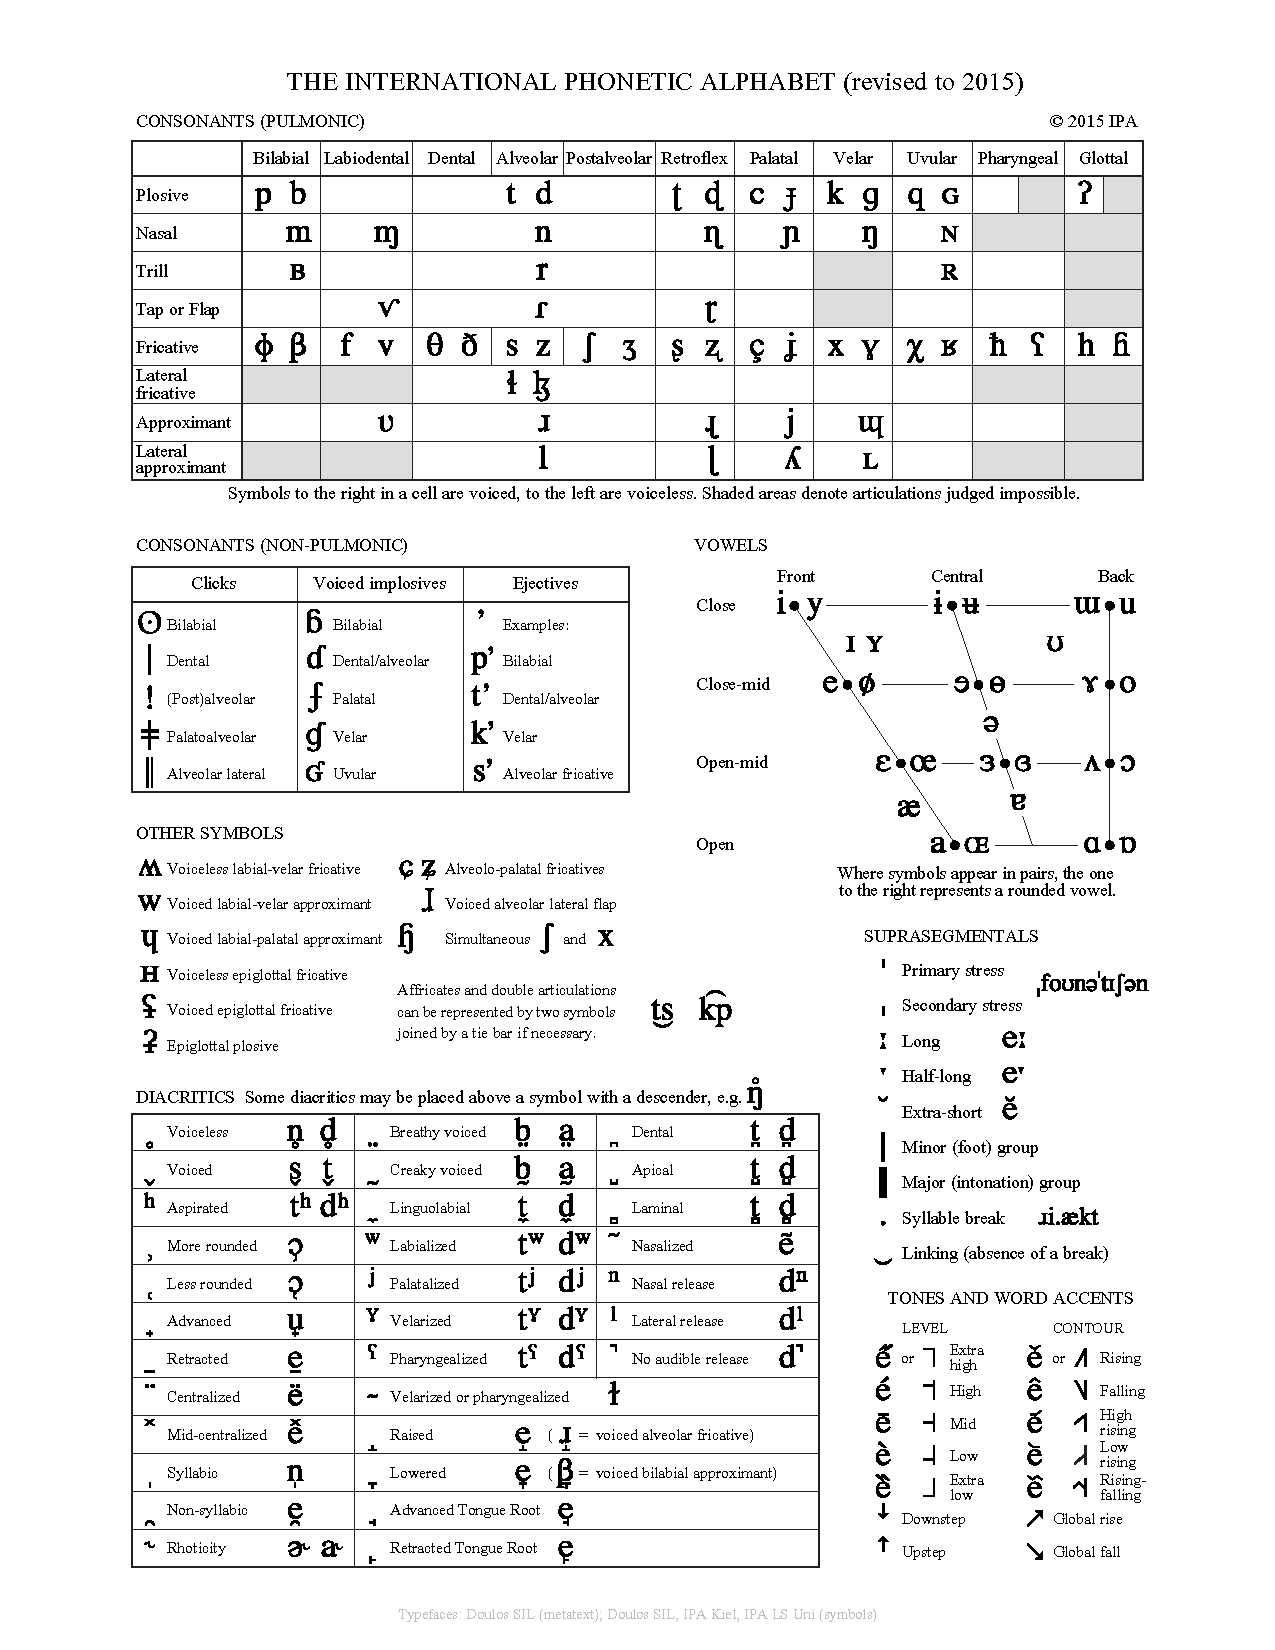
\includegraphics[width=1.3\linewidth]{ipa_chart.pdf}
    \end{center}
    \stepcounter{myfigure}
    \caption[Full IPA chart]{This is the full IPA chart, last updated in 2015}
    \label{fig:ipa_chart}
\end{figure}